% Makalenin 3 alt bölümü için 2x4 birleşik sonuç figürleri.
%
% Overleaf: fig_results_ISP.pdf, fig_results_VBW.pdf ve fig_results_VNode.pdf
% dosyalarını projedeki figures/ klasörüne yükleyin.
% Makaleye sadece "figure*" bloklarını kopyalayın; preamble'dan yalnızca
% graphicx ve \graphicspath satırı gerekir.
%
% figure*  : çift sütunlu şablonda iki sütuna yayılır (bu figürler için gerekli).
% Tek sütunlu şablonda "figure*" yerine "figure" yazın; width=\textwidth aynı kalır.

\documentclass[10pt,twocolumn]{article}
\usepackage[letterpaper,margin=0.67in]{geometry}
\usepackage{graphicx}
\graphicspath{{figures/}{./}}

\begin{document}

\section{Results}

\subsection{Effect of the Number of Switches per ISP}
Fig.~\ref{fig:results_isp} shows the results as the number of switches per ISP increases.

\begin{figure*}[!t]
    \centering
    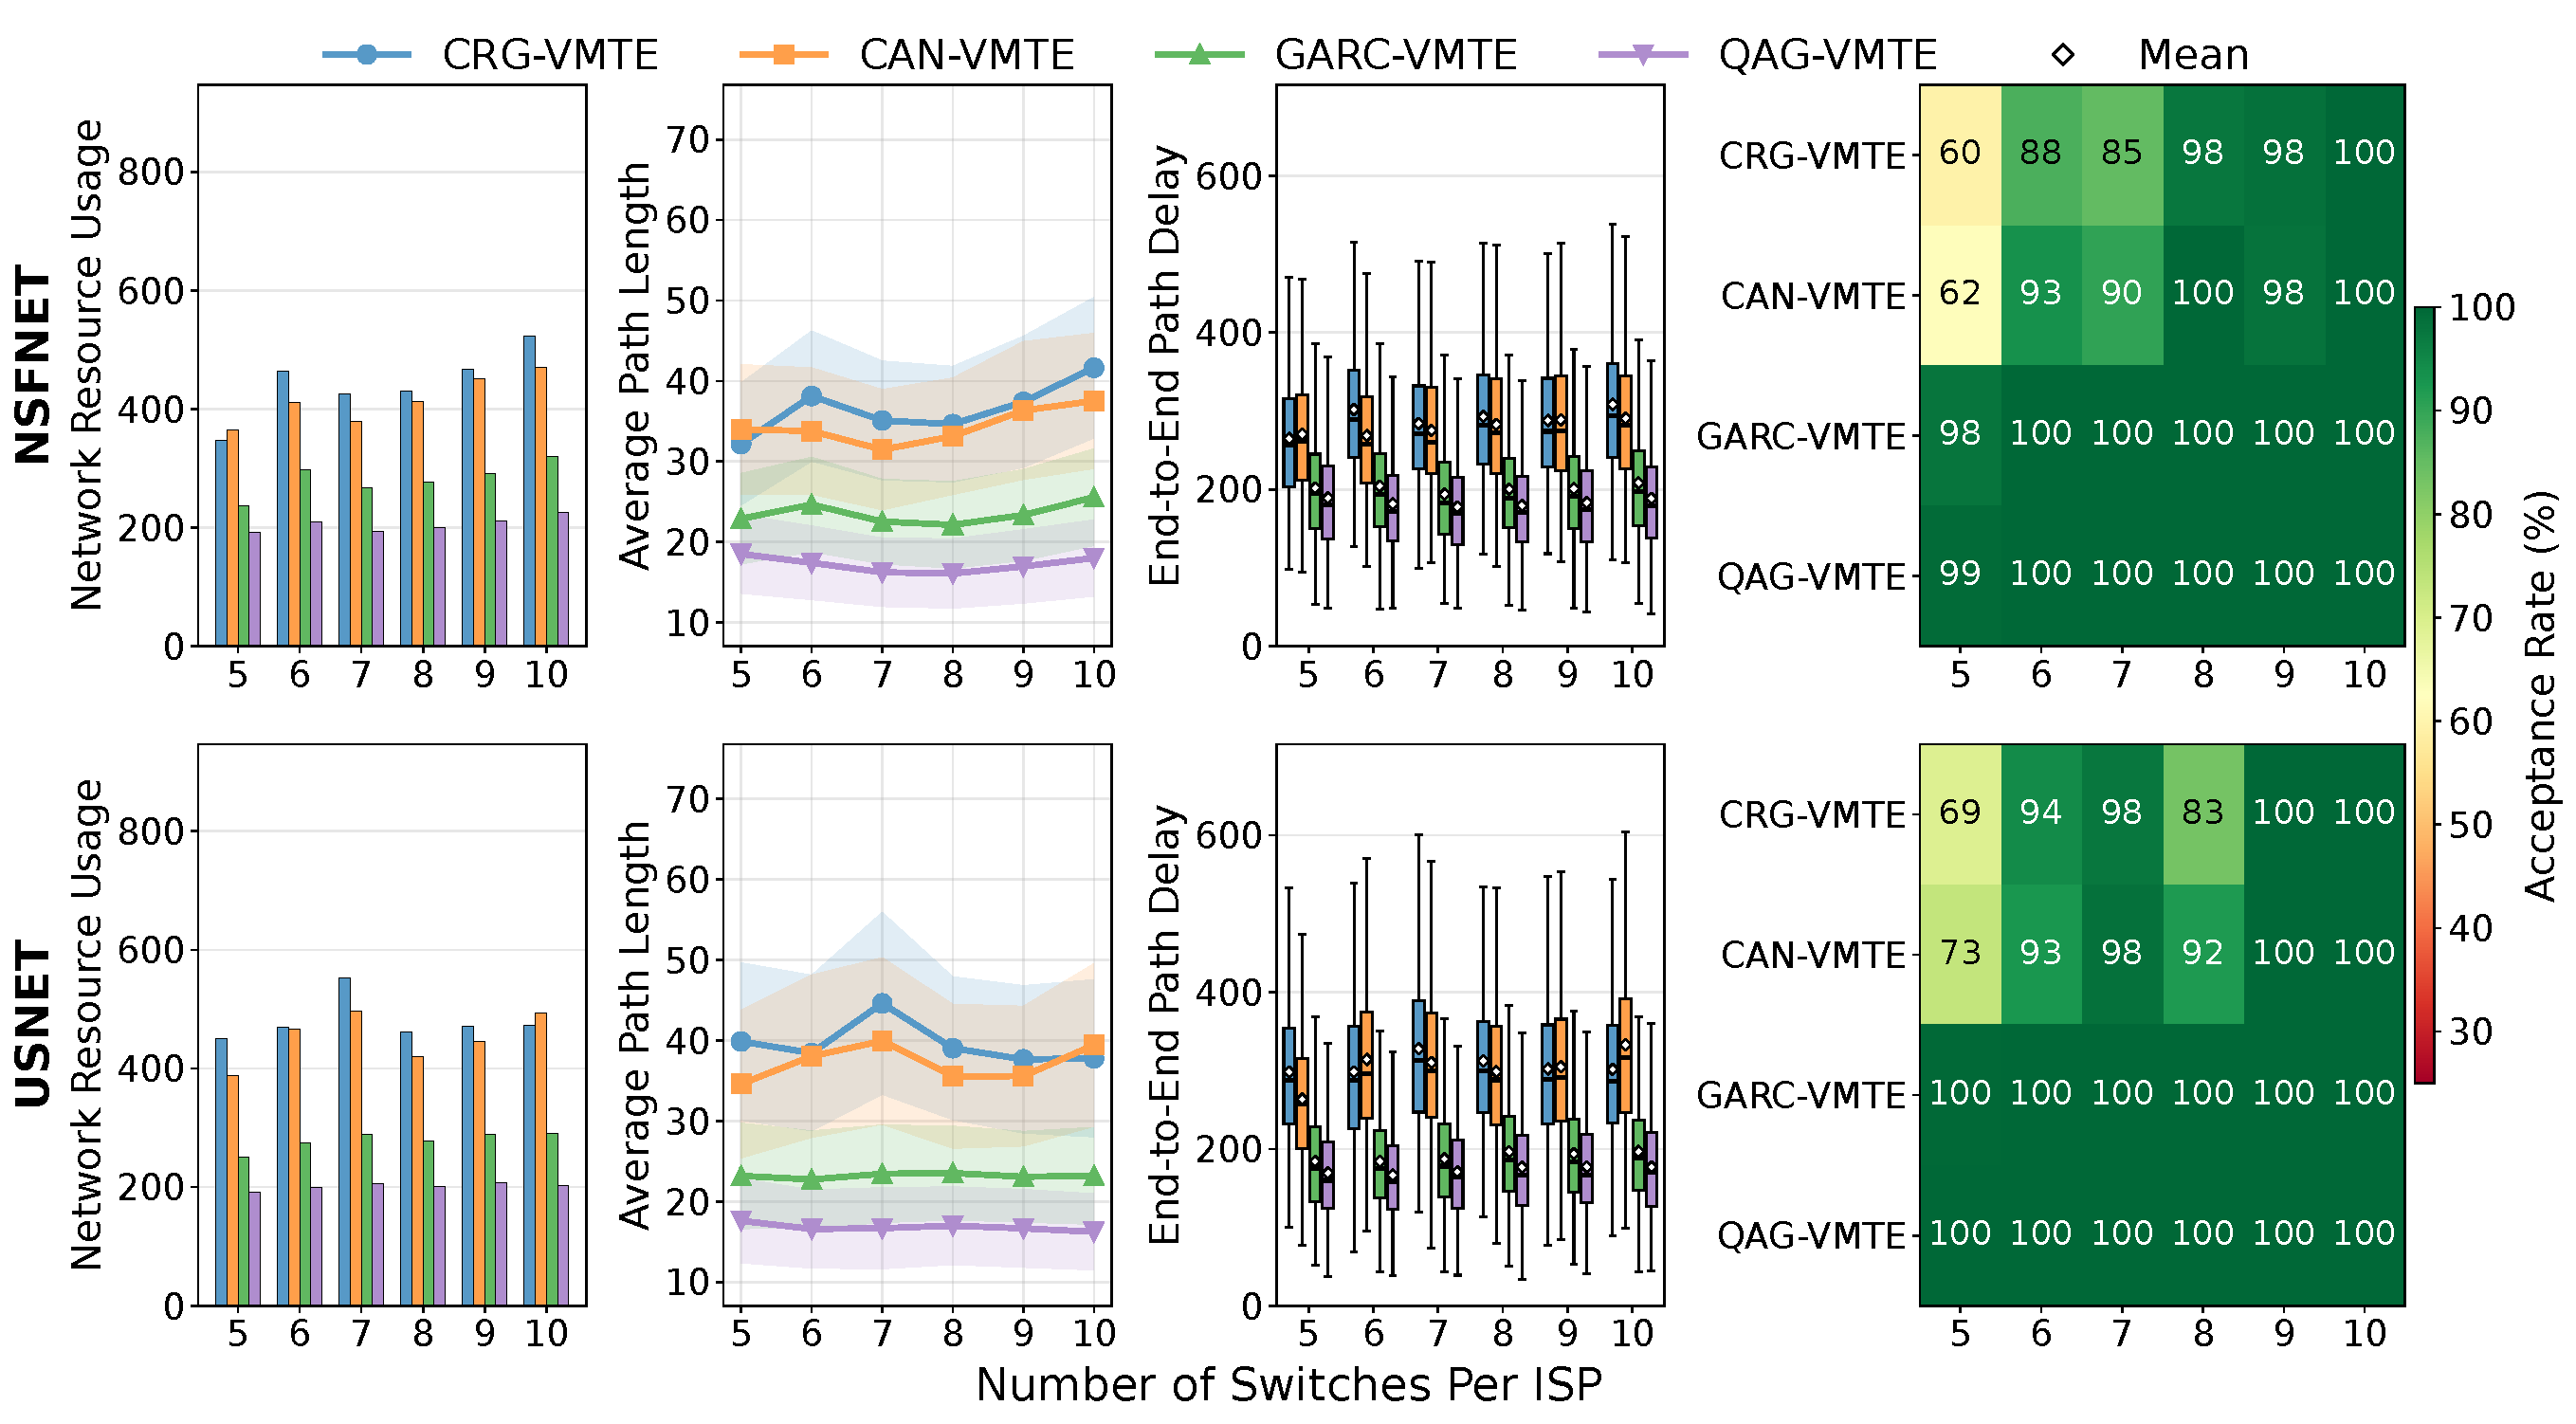
\includegraphics[width=\textwidth]{fig_results_ISP.pdf}
    \caption{Results for an increasing number of switches per ISP on NSFNET (top row)
    and USNET (bottom row), for requests with 6--8 virtual nodes and a bandwidth demand
    of 10 or 15. From left to right: network resource usage, computed over the requests
    accepted by all four algorithms; average path length, with shaded bands showing
    $\pm 1$ standard deviation; end-to-end path delay, with whiskers extending to
    $1.5\times$IQR and outliers omitted; and acceptance rate.}
    \label{fig:results_isp}
\end{figure*}

\subsection{Effect of the Bandwidth Demand}
Fig.~\ref{fig:results_vbw} shows the results as the bandwidth demand increases.

\begin{figure*}[!t]
    \centering
    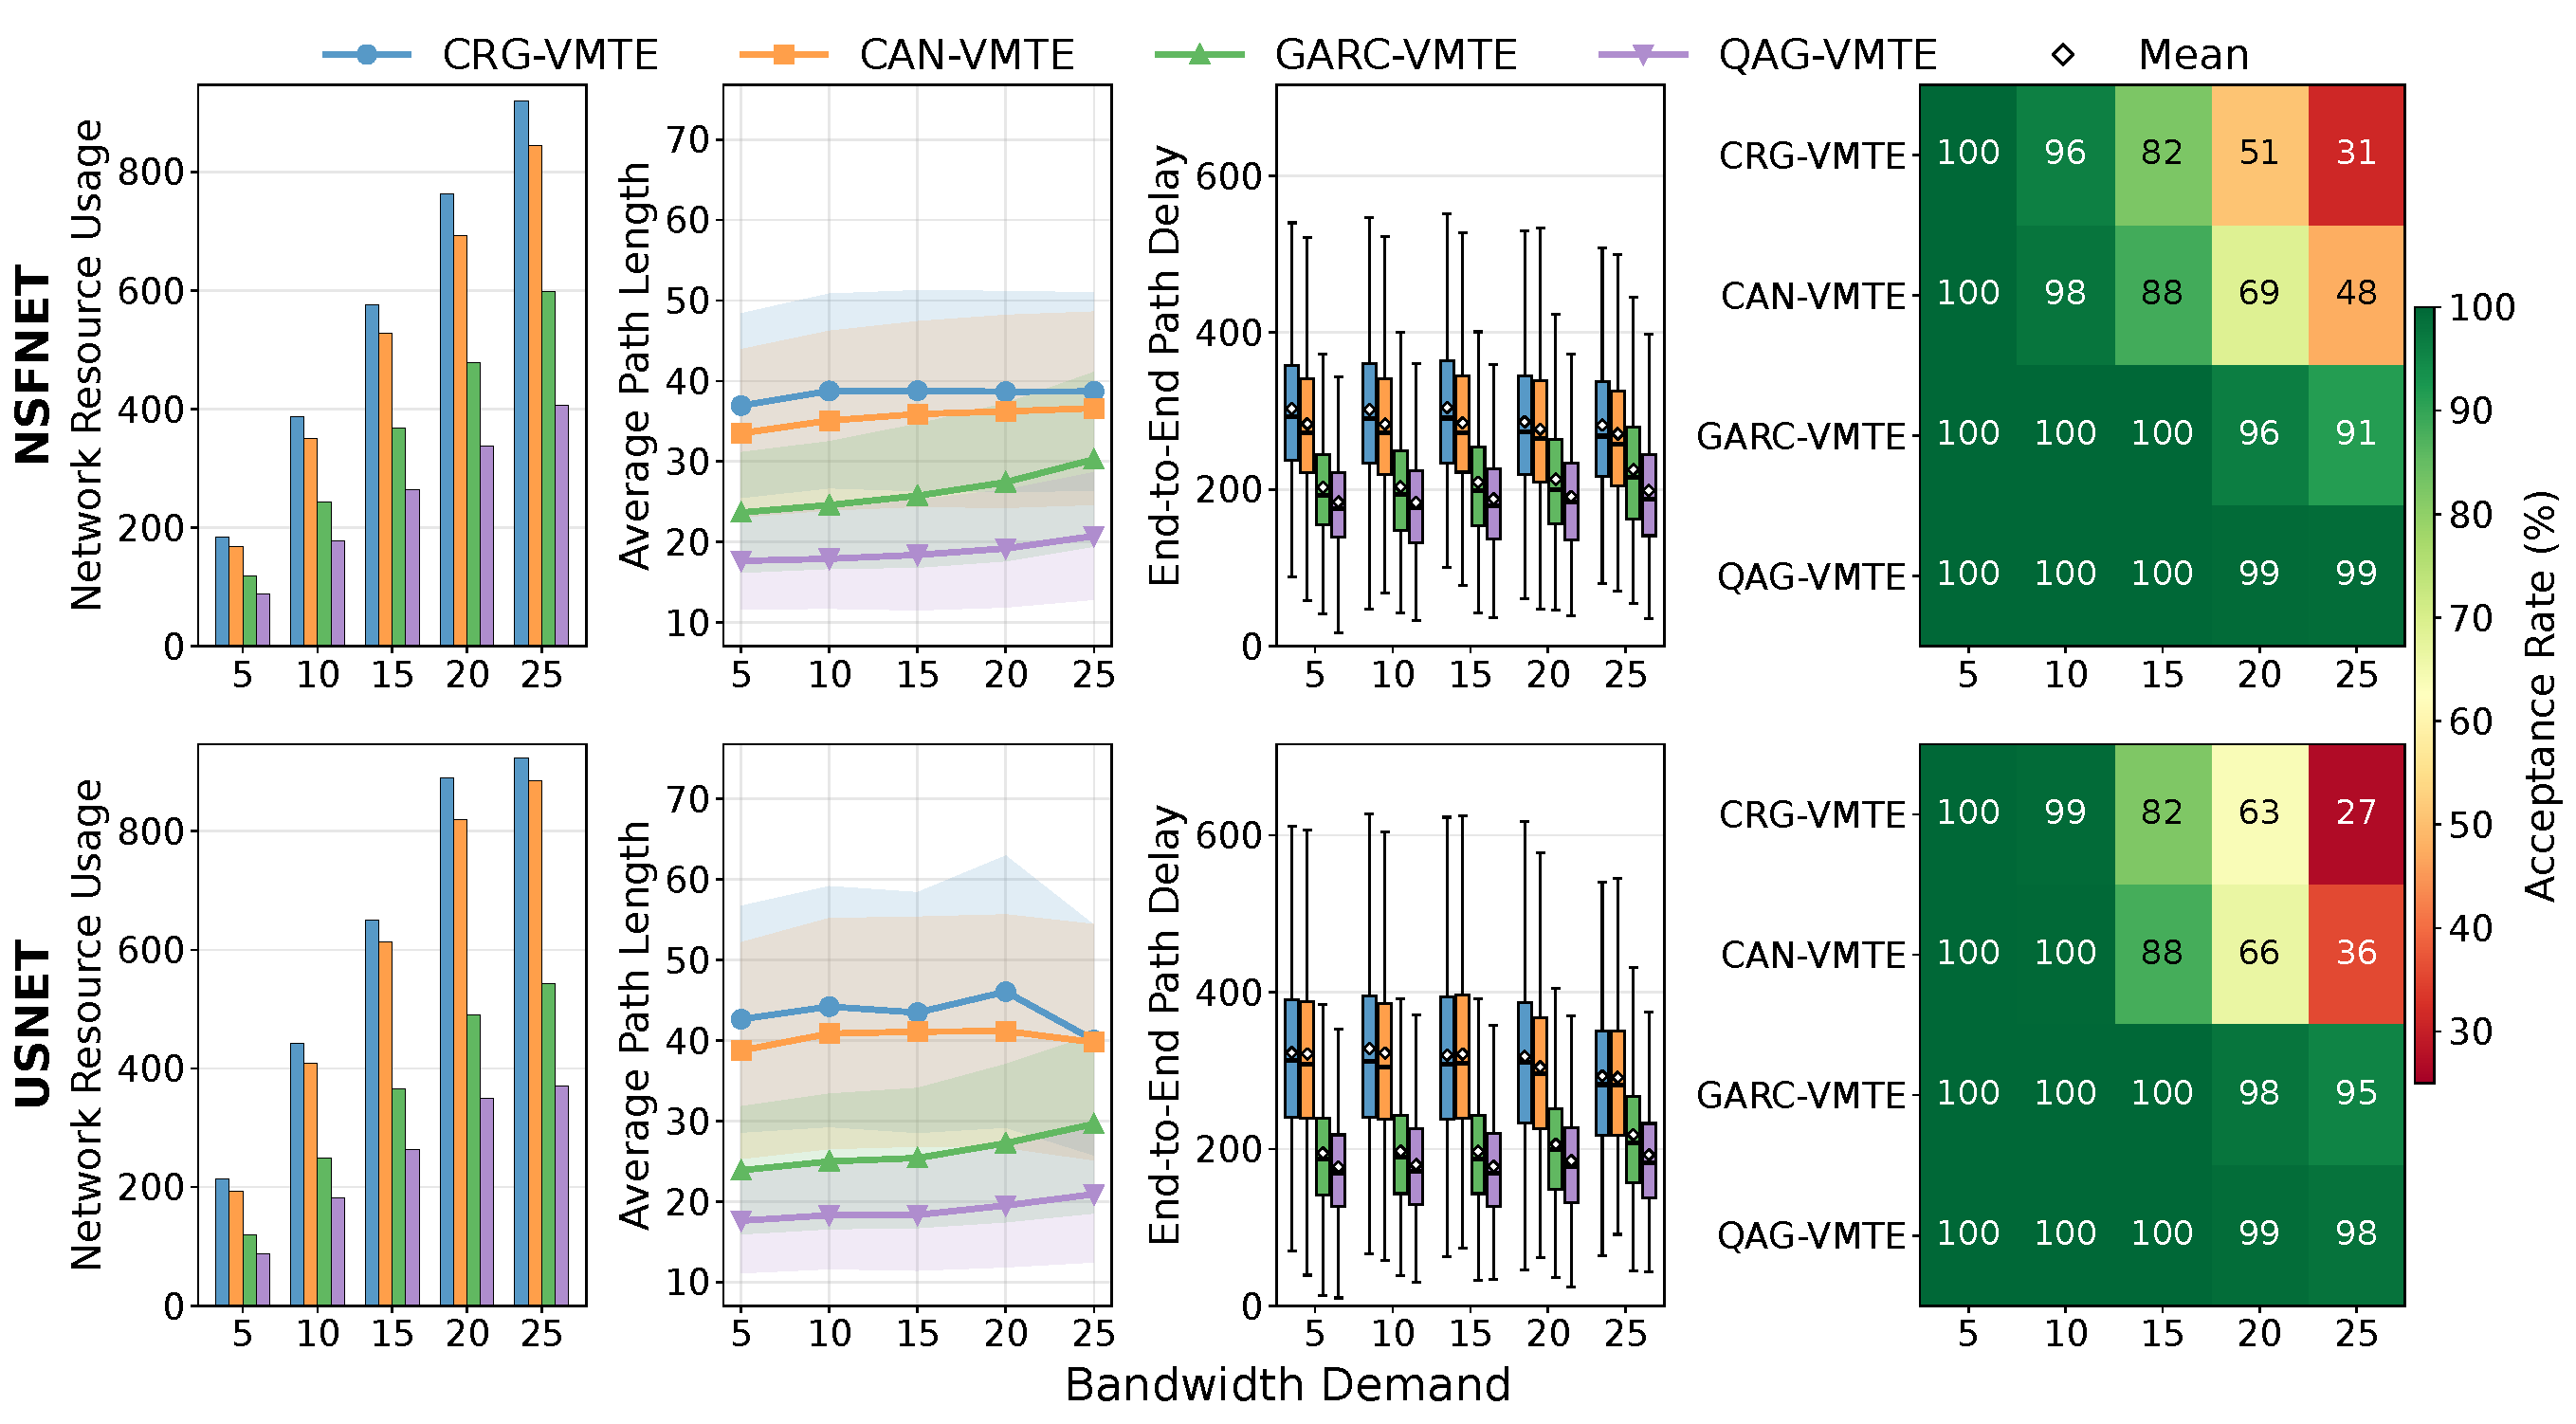
\includegraphics[width=\textwidth]{fig_results_VBW.pdf}
    \caption{Results for an increasing bandwidth demand on NSFNET (top row) and USNET
    (bottom row), aggregated over topologies with 6, 7 and 8 switches per ISP. The
    panels follow the same order and conventions as in Fig.~\ref{fig:results_isp}.}
    \label{fig:results_vbw}
\end{figure*}

\subsection{Effect of the Number of Virtual Nodes}
Fig.~\ref{fig:results_vnode} shows the results as the number of virtual nodes increases.

\begin{figure*}[!t]
    \centering
    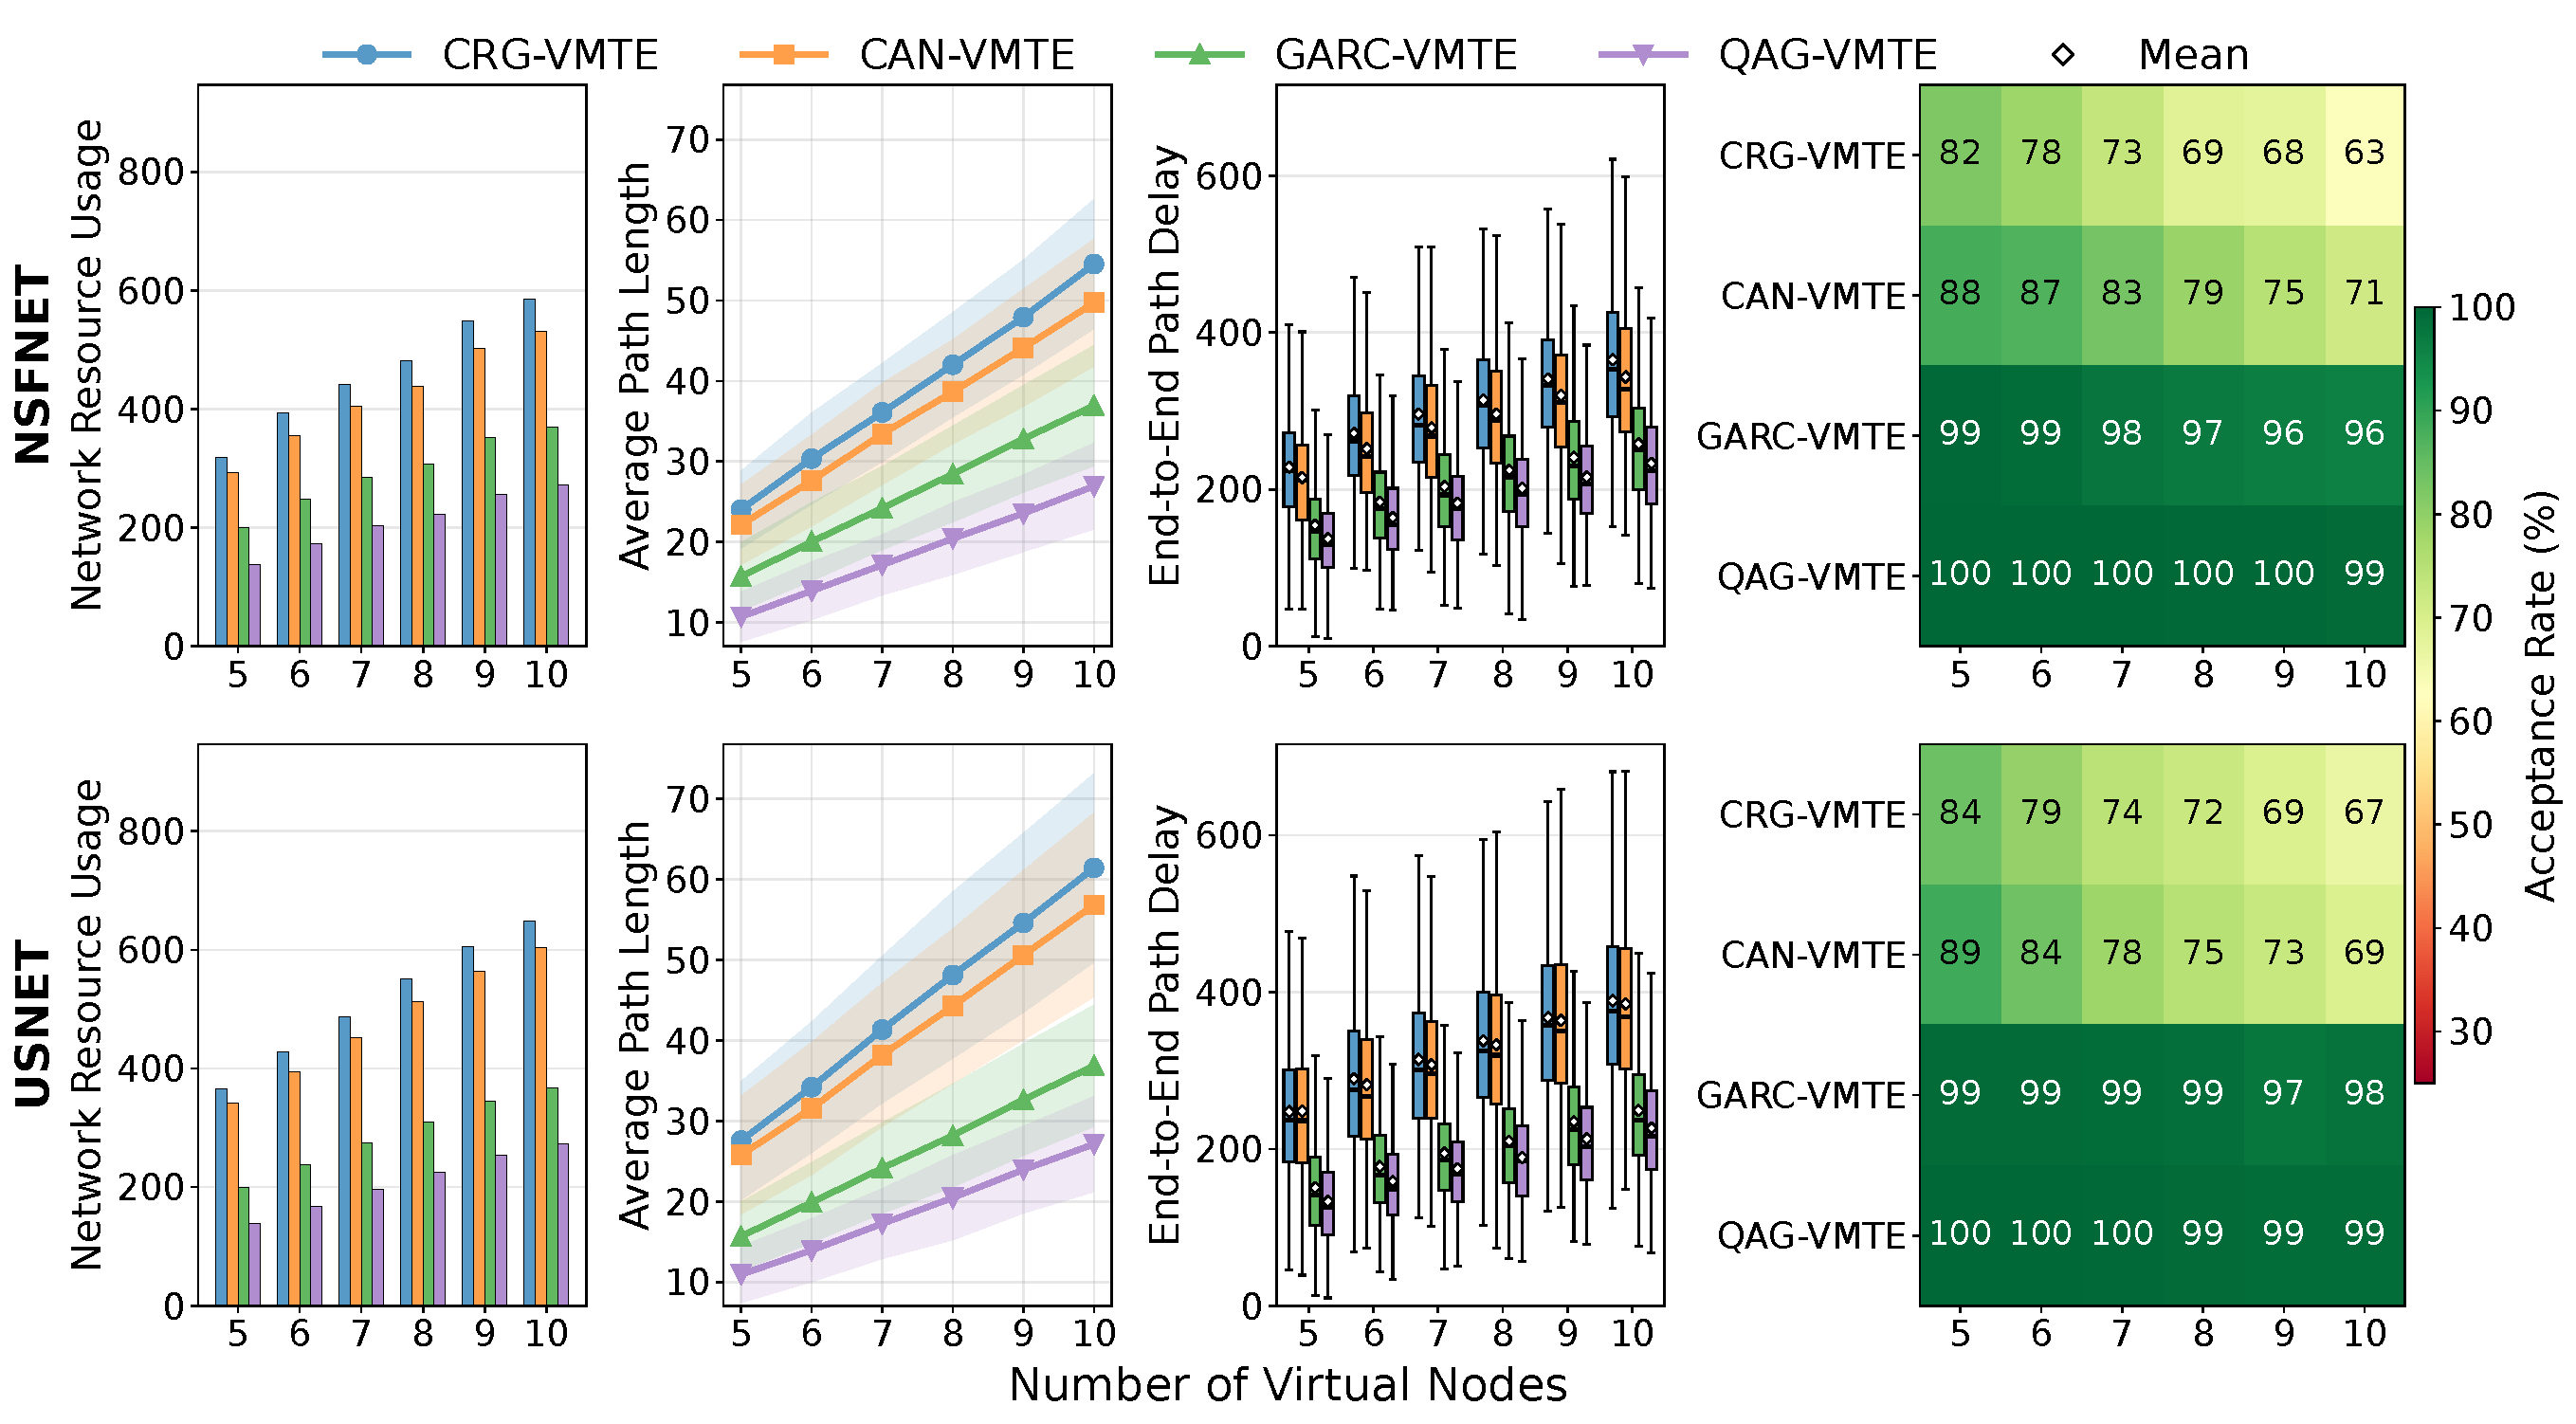
\includegraphics[width=\textwidth]{fig_results_VNode.pdf}
    \caption{Results for an increasing number of virtual nodes on NSFNET (top row) and
    USNET (bottom row), aggregated over topologies with 6, 7 and 8 switches per ISP. The
    panels follow the same order and conventions as in Fig.~\ref{fig:results_isp}.}
    \label{fig:results_vnode}
\end{figure*}

\end{document}
